% !TEX root = ../main.tex

\chapter{A Runtime Prediction Model}
\label{chap:model}
In this chapter, a runtime model for the execution of domain iterations on the GPU will be established. There are two components that need to be modeled for the runtime model. The first is the overhead for the transfer of memory to and from the GPU. For many computations, this will be a bottleneck, and the part of process the majority of the run time is spent on. It is discussed in detail in section \ref{sect:model_transfer}. The other part of the model deals with the execution of the kernel of the kernel on the GPU. Here, a number of parameters influence the execution time. These are discussed in section \ref{sect:model_runtime}.


\section{Memory Transfer Costs}
\label{sect:model_transfer}
Data for GPGPU computations need to be copied from the host to the device and back again. This process causes a significant runtime overhead, as the CPU and the GPU typically do not share the same memory resources. Hence, memory will need to be copied back and forth. In modern PCs, GPUs are typically connected to the CPU via the \textit{PCI Express 2.0} BUS\footnote{For example in the Chipset Architecture of the X79 Intel chipset \cite{intel2011x79}}. This bus offers a peak transfer performance of $1 \frac{GBit}{s}$ per lane. Typically, GPUs have 16 lanes available to them, in case of Multi-GPU systems or notebooks, only 8 lanes might be available for each GPU. For the latter\footnote{The author of the thesis performed most measurements using a Notebook GPU, hence it will be used for the examples given here.} case, this amounts to a theoretical performance of $1\frac{GB}{s}$. The RAM of the PC is also directly connected to the CPU. In the case of DDR3-SDRAM, the current state of memory technology, the theoretical maximum bandwidth would be between $6.4 - 17.1 \frac{GB}{s}$. This effectively makes the PCI Express bus a bottleneck when only considering the bandwidth. \cite{intel2011x79, schnabel2014ddr} \\

Another point to consider is latency. The signals on the BUS systems travel with a high but finite velocity. For printed circuit boards, this velocity is around half the speed of light, or about $150\frac{mm}{ns}$. With modern CPU and GPU architectures having clock rates of several GHz, several cycles may be needed for signals holding the request for data to reach the memory, and several more for the data to reach the GPU. Added to that is the is the latency of the memory module. For smaller memory segments, that combined latency is the defining factor in determining the time spent on copying memory. Measurements supporting this assertion can be found in \cite{fujii2013data} and in the measurements below in figure \ref{fig:model_gpu_transfer}. \cite{weiler2006guidelines, fujii2013data} \\

\begin{align}
	\label{eq:model_gpu_transfer}
	t_{trans}(x) &= b^{-1} * x + l_{prop}
\end{align}

The structure above makes it a reasonable assumption that the variable is the amount of memory  copied to and from the device. The propagation latency $l_{prop}$ is only observed once per transfer, which makes it a constant offset. The reciprocal of the bandwidth $b$ determines how many seconds it takes to copy one byte. It needs to be multiplied by the number of bytes copied. The result of this is described in equation \ref{eq:model_gpu_transfer}. To test this claim, a benchmark that copies data to and from the GPU was performed, and the time spent on both transfers was recorded. The results of these measurements are shown in figure \ref{fig:model_gpu_transfer}. It may be seen that there is significantly more time spent copying data to the GPU than on copying the results back again, although the size of the data remains the same. This effect is also  referred to in \cite{fujii2013data}. The details of the GPU architectures and the runtimes are not documented, however, and hence no explanation for the cause of the effect can be given. \\

\begin{figure}
	\begin{center}
		\begin{tikzpicture}
			\begin{axis}[	xlabel=Number of DWords, 
							ylabel=Time in µs,
							legend entries={To GPU, From GPU, To GPU interpolated, From GPU interpolated},
							legend style={at={(1.03, 0.5)}, anchor=west}]
				\addplot [blue, mark=halfcircle, error bars/.cd, y dir=both, y explicit] table [x=NumElements, y=ToGpu, y error=ToGpuStdDev]{data/copyGPUData.csv};
				\addplot [green, mark=halfcircle, error bars/.cd, y dir=both, y explicit] table [x=NumElements, y=FromGpu, y error=FromGpuStdDev]{data/copyGPUData.csv};
				\addplot [red, domain=1e3:67e6, samples=5] {0.00351162*x+516.413};
				\addplot [orange, domain=1e3:67e6, samples=5] {0.000537919*x+173.626};
			\end{axis}
		\end{tikzpicture}
		\caption{Transfer times for memory. Time spent copying to the GPU is shown in blue, and time spent copying from the GPU is shown in green.}
		\label{fig:model_gpu_transfer}
	\end{center}
\end{figure}

From the values of figure \ref{fig:model_gpu_transfer}, formulae for the transfer times of host-to-device (equation \ref{eq:model_gpu_transfer_to}) and device-to-host (equation \ref{eq:model_gpu_transfer_from}) can be derived. For the test device, a linear interpolation yields the following data:

\begin{align}
	\label{eq:model_gpu_transfer_to} t_{\rightarrow GPU_{rMBP}} &= 0.00357997\mu s * x + 516.413\mu s\\
	\label{eq:model_gpu_transfer_from} t_{\leftarrow GPU_{rMBP}} &= 0.00053337\mu s * x + 173,626\mu s
\end{align}

Equations \ref{eq:model_gpu_transfer_to} and \ref{eq:model_gpu_transfer_from} are also shown in figure \ref{fig:model_gpu_transfer}. One might observe that the linear structure of the model described above fits well with the data gathered experimentally.

\newpage


%%%%%%%%%%%%%%%%%%%%%%%%%%%%%%%%%%%%%%%%%%%%%%%%%%%%%%%%%%%
\section{Base Cost for Running Kernels}
\label{sect:model_runtime}
As previously noted, computations on the GPU are performed in a massively parallel fashion, with each work item being computed in its own thread. These threads need to be started, categorized and put into thread blocks, which might cause a noticeable amount of overhead. To measure the costs, an empty kernel that only queries its own id is executed, with a different number of work items being tested. The kernel can be seen in \ref{sect:appendix_opencl_empty}. It is basically an empty kernel, except for the function call to inquire the id of the work item the kernel is executed on. This operation has to be performed whenever a kernel is executed, as it has to be used to determine which element in the memory should be accessed. \\

\begin{figure}[h]
	\begin{center}
		\begin{tikzpicture}
			\begin{axis}[	xlabel=Number of Elements, 
							ylabel=Time in µs,
							legend entries={Empty Kernel Runtime, Interpolated Function},
							legend style={at={(1.03, 0.5)}, anchor=west}]
				\addplot [blue, error bars/.cd, y dir=both, y explicit] table [x=NumberOfElements, y=Runtime, y error=StandardDeviation]{data/emptyKernel.csv};
				\addplot [red, domain=1e3:16.7e6, samples=5] {0.000189885660433182 * x + 5.72651881044402};
			\end{axis}
		\end{tikzpicture}
		\caption{Execution time for empty Kernels. The experimentally gathered data points are shown in blue, and the Interpolated Function is shown in red.}
		\label{fig:model_empty_kernel}
	\end{center}
\end{figure}

As it can be seen here, the runtime scales linearly against the number of work items that are executed on the GPU. With that in mind the function $T_{Base}$ (see equation \ref{eq:model_empty_kernel}) for the runtime of empty kernels may be assigned for the run time of empty kernels. Equation \ref{eq:model_empty_kernel_mbp} shows a sample assignment of the values based upon the results of the benchmarks executed on the GT-650M.

\begin{align}
	\label{eq:model_empty_kernel} T_{Base}(x) &= t_{Element}*x+c \\
	\label{eq:model_empty_kernel_mbp}T_{Base_{rMBP}} &= 0.18988566ns * x + 5.72652\mu s
\end{align}

\newpage



%%%%%%%%%%%%%%%%%%%%%%%%%%%%%%%%%%%%%%%%%%%%%%%%%%%%%%%%%%%
\section{Influence of the Work-Group Size}
\label{sect:model_wgsize}

In OpenCL, work items are grouped into so-called \textit{work-groups}. Each work-group has the same number of work items. The total number of work items has to be divisible by the work-group size. Work-groups are executed in sequence. Once all work items within a  work-group have finished executing, the execution of work items belonging to the next work-group will be started. From this follows that the work-group needs to be sufficiently large in order to utilize all the available processors on the GPU. Additionally, if the number of work items within a work-group is sufficiently large, the scheduler will employ techniques to hide the latency of loading data from the off-chip global memory. \cite{khronos2012specification,nvidia2009opencl}\\

To evaluate this behavior, another benchmark has been implemented. In this case, the kernel in question (shown in section \ref{sect:appendix_opencl_wg} in the appendix) is executed with a varying work-group size on an array with roughly $2^{20}$ elements. The imprecision is due to the fact that the work-groups need to be an even divider of the total number of work items. At that number of elements the amount of memory will vary by only 0.1\%, which makes the impact of the memory size negligible. \\

\begin{figure}[p]
	\begin{center}
		\begin{tikzpicture}
			\begin{axis}[	xlabel=Number of work items per work-group, 
							ylabel=Time in µs,
							legend entries={Kernel Runtime, Interpolated Function},
							legend style={at={(1.03, 0.5)}, anchor=west}]
				\addplot [green] table [x=WorkgroupSize, y=Runtime]{data/wgSize.csv};
				\addplot [red, domain=1:1e3, samples=500] {18192*exp(-x/12.2112414869873)+36412*exp(-x/2.28329383738342)+1395.1};
			\end{axis}
		\end{tikzpicture}
		\caption{Execution time for different work-group sizes. The experimentally-gathered data is shown in green, the Interpolated Function in red.}
		\label{fig:model_wgsize}
	\end{center}
\end{figure}

The data obtained by executing the test, shown in figure \ref{fig:model_wgsize} validates the claims made above. For the GPU the benchmark was executed on, there is a severe speed penalty when working with a work-group size below sixteen. In the worst case with a work-group only containing a single work item, the execution time is higher by a factor of fifty compared to using the maximum number of work-items in a work-group. With sixteen to one hundred work items in a work-group, there is still a significant decrease in execution time for bigger work-groups. Above this, no more significant increases in execution speed were observed. \\

From the data obtained, the formula given in equation \ref{eq:model_wgsize} can be deduced. It is a sum of two inverse exponential functions. The subexpression denoted as \textbf{A} marks the influence resource utilization has on the program. The subexpression denoted as \textbf{B} shows a decline that is less steep than the first. It models the influence the scheduler has on the execution time. Equation \ref{eq:model_wgsize_mbp} shows a concrete assignment of the variables using the data obtained from the benchmark.

\begin{figure}[p]
	\begin{center}
		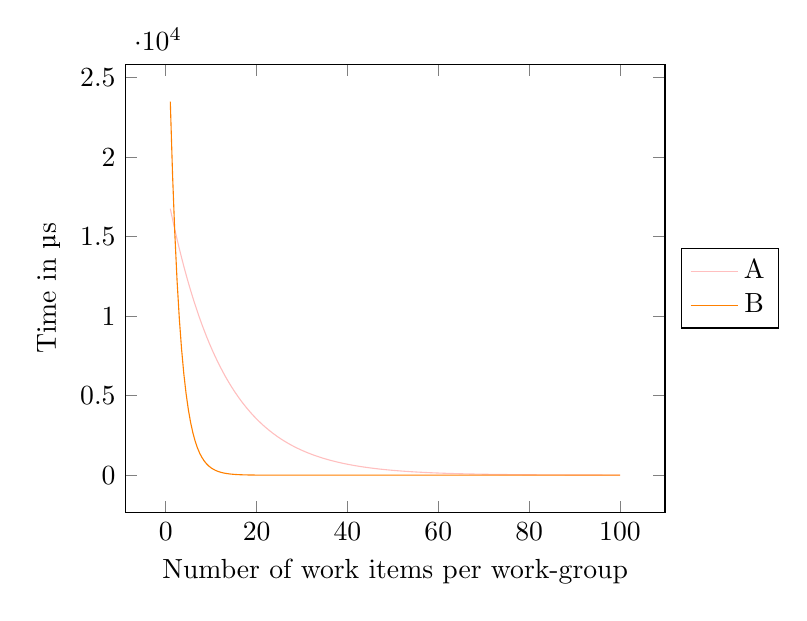
\begin{tikzpicture}
			\begin{axis}[	xlabel=Number of work items per work-group, 
							ylabel=Time in µs,
							legend entries={A,B},
							legend style={at={(1.03, 0.5)}, anchor=west}]
				\addplot [pink, domain=1:100, samples=200] {18191.5547276*exp(-x/12.2112414869873)};
				\addplot [orange, domain=1:100, samples=200] {36411.9660021091*exp(-x/2.28329383738342)};
			\end{axis}
		\end{tikzpicture}
		\caption{The two different components of the function \ref{eq:model_wgsize} derived from the data given in figure \ref{fig:model_wgsize}.}
		\label{fig:model_wgsize_components}
	\end{center}
\end{figure}
\begin{align}
\label{eq:model_wgsize} M_{WG}(x) &= \underbrace{B_1*e^{\frac{-x}{t_1}}}_\text{A} + \underbrace{B_2*e^{\frac{-x}{t_2}}}_\text{B}+y_0\\
\label{eq:model_wgsize_mbp} M_{WG_{rMBP}}(x) &= 13.04 * e^{\frac{-x}{12.21124}} + 26.10 * e^{\frac{-x}{2.28329}}
\end{align}

\newpage


%%%%%%%%%%%%%%%%%%%%%%%%%%%%%%%%%%%%%%%%%%%%%%%%%%%%%%%%%%%
\section{Basic Operations}
\label{sect:model_ops}
The four basic operations, $+$, $-$, $*$ and $/$, are discussed here as applied to various types of data, such as floating point values and integers. The documentation of the NVidia OpenCL platform gives some estimates about the projected performance, specifying how many operations can be completed per clock cycle. This metric is established by looking at a single SIMT-Element (warp) with 32 elements, which synchronously executes one instruction comprising of 32 operations. One may examine the number of cycles a warp takes to be executed, and hence deduce the operations throughput from this. \cite{nvidia2009opencl} \\

According to the documentation, for Additions, Subtractions and Multiplications of floating point numbers, throughput is identical at \textbf{8} operations per clock cycle. Division should be slower, at \textbf{0.88} operations per cycle. For integer arithmetic, Addition and Subtraction are at \textbf{8} operations per cycle. Multiplication of integers should be slower, at \textbf{2} operations per cycle, and Division and Modulo are slower again. In case of literals, the compiler will try to replace the Division and Modulo by Bit-Shifts or Bitwise AND-Operations. A single Bit-Shift or AND-Operation should again be at \textbf{8} operations per cycle. The actual performance benefit depends upon the literal.\cite{nvidia2009opencl} \\

To evaluate these claims, another benchmark was implemented. The variable, once again, is the size of the memory segment that is iterated upon. Tests are conducted for the four basic operation types, both for floating point and integer arithmetic. This alone would not suffice to deduce the time spent on the operations, however, as it is not possible to write a kernel that only performs a single basic operation. For example, there always is the base cost discussed earlier, and a memory accesses to save the result is needed so the compiler does not eliminate the operation. To mitigate this, first a benchmark that only performs a read and a write was executed, and the runtime difference between that one and the benchmark with the basic operations is deducted to be the time spent on the operation. The kernels used for the benchmark are shown in section \ref{sect:appendix_opencl_ops_single} in the appendix. \\
 
\begin{figure}[p]
	\begin{center}
		\begin{tikzpicture}
			\begin{axis}[	xlabel=Number of Elements, 
							ylabel=Time in µs,
							legend entries={ADD, SUB, MUL, DIV},
							legend style={at={(1.03, 0.5)}, anchor=west}]
				\addplot [blue, error bars/.cd, y dir=both, y explicit] table [x=NumElements, y=Add]{data/singleFloat.csv};
				\addplot [green, error bars/.cd, y dir=both, y explicit] table [x=NumElements, y=Sub]{data/singleFloat.csv};
				\addplot [red, error bars/.cd, y dir=both, y explicit] table [x=NumElements, y=Mul]{data/singleFloat.csv};
				\addplot [orange, error bars/.cd, y dir=both, y explicit] table [x=NumElements, y=Div]{data/singleFloat.csv};

			\end{axis}
		\end{tikzpicture}
		\caption{Execution time for basic operations on floating point values. The Standard Deviation is omitted from this diagram for legibility reasons. For diagrams containing the Standard Deviation, see figure \ref{fig:model_ops_single_float_add} (Addition), figure \ref{fig:model_ops_single_float_sub} (Subtraction), figure \ref{fig:model_ops_single_float_mul} (Multiplication) and figure \ref{fig:model_ops_single_float_div} (Division) in the appendix.}
		\label{fig:model_ops_single_float}
	\end{center}
\end{figure}

\begin{figure}[p]
	\begin{center}
		\begin{tikzpicture}
			\begin{axis}[	xlabel=Number of Elements, 
							ylabel=Time in µs,
							legend entries={ADD, SUB, MUL, DIV},
							legend style={at={(1.03, 0.5)}, anchor=west}]
				\addplot [blue, error bars/.cd, y dir=both, y explicit] table [x=NumElements, y=Add]{data/singleInt.csv};
				\addplot [green, error bars/.cd, y dir=both, y explicit] table [x=NumElements, y=Sub]{data/singleInt.csv};
				\addplot [red, error bars/.cd, y dir=both, y explicit] table [x=NumElements, y=Mul]{data/singleInt.csv};
				\addplot [orange, error bars/.cd, y dir=both, y explicit] table [x=NumElements, y=Div]{data/singleInt.csv};

			\end{axis}
		\end{tikzpicture}
		\caption{Execution time for basic operations on integer values. The Standard Deviation is omitted from this diagram for legibility reasons. For diagrams containing the Standard Deviation, see figure \ref{fig:model_ops_single_int_add} (Addition), figure \ref{fig:model_ops_single_int_sub} (Subtraction), figure \ref{fig:model_ops_single_int_mul} (Multiplication) and figure \ref{fig:model_ops_single_int_div} (Division) in the appendix.}
		\label{fig:model_ops_single_int}
	\end{center}
\end{figure}

The data from the benchmark (figure \ref{fig:model_ops_single_float}) shows that for floating point arithmetic, only use of the division causes a significant computational overhead. The other operations seem to be behaving identically, causing next to no overhead at all. This is more or less in line with the NVidia OpenCL programming guide\footnote{see \cite{nvidia2009opencl}}. However, the evaluation of the model revealed the costs spent on the division operation to be smaller in most cases. This effect is discussed in section \ref{sect:future_model}.\\ 

For integer operations (figure \ref{fig:model_ops_single_int}), the division is also the slowest operation. The other operations are running at a similar speed. A speed difference between Additions and Subtractions on the one side, and Multiplication on the other could not be reproduced with this benchmark. It was observed that the floating point division is much slower then its integer division counterpart, presenting a stark contrast to the information given in the NVidia OpenCL programming guide. \\

Nevertheless, the run times for each operation are observed mostly to scale linearly with the number of elements that have to be computed. Hence, the equations that model the runtime were extracted from the data of the benchmarks, yielding the equations \ref{eq:model_ops_single} as a result.

\begin{align}
\label{eq:model_ops_single}
T^{Op}_{type}(x) &= t_{Element}*x+c\\
T^{+}_{float}(x) &= 3.2679908306701 ps*x\notag\\
T^{-}_{float}(x) &= 4.42040597789466 ps*x\notag\\
T^{*}_{float}(x) &= 4.44336371720927 ps*x\notag\\
T^{/}_{float}(x) &= 0.000586512010350116\mu s*x+2.28467688281392\mu s\notag\\
T^{+}_{int}(x) &= 3.28593145810764 ps*x\notag\\
T^{-}_{int}(x) &= 6.1655964896141 ps*x\notag\\
T^{*}_{int}(x) &= 4.83050202348605 ps*x\notag\\
T^{/}_{int}(x) &= 8.97819795983561 * 10^{-2}ns*x+3.02532315741367\mu s\notag
\end{align}

\subsection{Multiple Basic Operations Per Kernel}
\label{sect:model_ops_multiple}
Tests conducted while just using the results from the previous sections and scaling them linearly did not produce accurate predictions. This became especially apparent on tests performed with kernels that contain multiple floating point divisions, as they have the most significant computational overhead. To investigate this effect, another benchmark was devised. This time, the size of the memory segment is held the same, at 256kB, and the number of operations that are to be executed on the data is varied. The kernel is shown in section \ref{sect:appendix_opencl_ops_multiple} in the appendix. \\

\begin{figure}[h]
	\begin{center}
		\begin{tikzpicture}
			\begin{axis}[	xlabel=Number of Operations, 
							ylabel=Time in µs,
							legend entries={ADD, SUB, MUL, DIV},
							legend style={at={(1.03, 0.5)}, anchor=west}]
				\addplot [blue, error bars/.cd, y dir=both, y explicit] table [x=NumOps, y=Add]{data/multipleInt.csv};
				\addplot [green, error bars/.cd, y dir=both, y explicit] table [x=NumOps, y=Sub]{data/multipleInt.csv};
				\addplot [red, error bars/.cd, y dir=both, y explicit] table [x=NumOps, y=Mul]{data/multipleInt.csv};
				\addplot [orange, error bars/.cd, y dir=both, y explicit] table [x=NumOps, y=Div]{data/multipleInt.csv};

			\end{axis}
		\end{tikzpicture}
		\caption{Total execution time for multiple basic operations on integer values. The x axis denotes the number of operations of a single type that are executed within a single kernel. The Standard Deviation is omitted for legibility reasons. In this case, it is fairly large, about $\pm50\mu s$ for the memory size of 256kB.}
		\label{fig:model_ops_multiple_int}
	\end{center}
\end{figure}

For integer arithmetics, the benchmark (see figure \ref{fig:model_ops_multiple_int}) reveals that for the basic operations, no noticeable difference was observed in how many operations of a particular type are performed in a kernel. A notable exception is the division operation. The compiler seems to be able to infer that if there are a certain number of divisions by a literal performed in sequence on the same number, the result will always be zero. In this case it can be eliminated\footnote{In the benchmark, divisions by seven are used, and $c \in \operatorname{int} \implies c / 7^{12} = 0$. Also, $7^{12}$ does not overflow, as the operations are applied sequentially.}. \\

Floating point arithmetic behave slightly differently. For Addition, Subtraction and Multiplication no increase in run time may be observed for the first few operations, and after that a slight increase with each added operation can be observed. That delay before the increase may be due to the program being memory-bound. With few operations, these can be executed whilst other threads are waiting for the memory access to be completed. \\

Divisions behave more erratically. Figure \ref{fig:model_ops_multiple_float_div} shows that the first two operations seem to adhere to the cost model deduced and shown in section \ref{sect:model_ops}, but afterwards they start taking longer to complete, and then, subsequent to 64 operations, they become even more expensive than before. The first two operations can be explained with the memory read shadowing the cost of the operation. The real cost of the operation becomes apparent afterwards. The second inflexion is not clear, however. \\

For the Addition, Subtraction and Multiplication, the formula \ref{eq:model_ops_multiple_float} can be derived. It takes the number of operations as input, and returns a multiplier to be applied to the linear runtime in order to get the final runtime. For $x$ values smaller than a threshold, the formula will return a multiplier that returns the runtime of a single operation. If $x$ is above the threshold, the formula will return the multiplier that takes the shadowed operations into account. This multiplier will gradually get closer to one as the number of operations that are shadowed, $x_{sat}$, gets smaller compared to the total number of operations performed in the kernel.

\begin{gather}
	\label{eq:model_ops_multiple_float}
	M(x) = 	\begin{cases}
				\frac{1}{x} & (x \leq x_{sat})\\
				\frac{x_{sat} - x}{x} & (x < x_{sat})
			\end{cases}
\end{gather} 

\begin{figure}[p]
	\begin{center}
		\begin{tikzpicture}
			\begin{axis}[	xlabel=Number of Operations, 
							ylabel=Time in µs,
							legend entries={ADD, SUB, MUL},
							legend style={at={(1.03, 0.5)}, anchor=west}]
				\addplot [blue, error bars/.cd, y dir=both, y explicit] table [x=NumOps, y=Add]{data/multipleFloat.csv};
				\addplot [green, error bars/.cd, y dir=both, y explicit] table [x=NumOps, y=Sub]{data/multipleFloat.csv};
				\addplot [red, error bars/.cd, y dir=both, y explicit] table [x=NumOps, y=Mul]{data/multipleFloat.csv};
			\end{axis}
		\end{tikzpicture}
		\caption{Total execution time for multiple basic operations (ADD, SUB, MUL) on floating point values. The x axis denotes the number of operations of a single type that are executed within a single kernel. The Standard Deviation is omitted for legibility reasons. In this case, it is fairly small, about $\pm10\mu s$ for the memory size of 256kB.}
		\label{fig:model_ops_multiple_float}
	\end{center}
\end{figure}
\begin{figure}[p]
	\begin{center}
		\begin{tikzpicture}
			\begin{axis}[	xlabel=Number of Operations, 
							ylabel=Time in µs,
							legend entries={DIV},
							legend style={at={(1.03, 0.5)}, anchor=west}]
				\addplot [red, error bars/.cd, y dir=both, y explicit] table [x=NumOps, y=Div, y error=DivStdDev]{data/multipleFloat.csv};
			\end{axis}
		\end{tikzpicture}
		\caption{Total execution time for multiple basic operations on floating point values. The x axis denotes the number of divisions that are executed within a single work item.}
		\label{fig:model_ops_multiple_float_div}
	\end{center}
\end{figure}

\newpage


%%%%%%%%%%%%%%%%%%%%%%%%%%%%%%%%%%%%%%%%%%%%%%%%%%%%%%%%%%%
\section{Memory Accesses}
\label{sect:model_access}
As already discussed in section \ref{sect:theory_opencl_memory}, there is a memory hierarchy in OpenCL. Recall that there are four different kinds of memory, \textit{private}, \textit{local}, \textit{constant}, and \textit{global}. Global memory is most expensive, with access incurring a cost of about 300 cycles. It is shared amongst all work items. Local memory is shared amongst the work items belonging to the same work-group. It typically offers a faster access speed compared to global memory. Private memory is used for local variables, and is private to one work item. It is typically very fast, most likely implemented as a register. The initial Benchmark uses a benchmark without a memory access as the base line, and compares the times spent on the private access, the local access and the global access. Again, the variable is the size of the array the kernel is executed upon. \cite{nvidia2008cuda}\\

\begin{figure}[hbp]
	\begin{center}
		\begin{tikzpicture}
			\begin{axis}[	xlabel=Number of Elements, 
							ylabel=Time in µs,
							legend entries={Private Access, Global Access, Local Access},
							legend style={at={(1.03, 0.5)}, anchor=west}]
				\addplot [blue, error bars/.cd, y dir=both, y explicit] table [x=NumberOfElements, y=private_access, y error=private_StdDev]{data/singleAccess.csv};
				\addplot [red, error bars/.cd, y dir=both, y explicit] table [x=NumberOfElements, y=global_write, y error=write_StdDev]{data/singleAccess.csv};
				\addplot [green, error bars/.cd, y dir=both, y explicit] table [x=NumberOfElements, y=just_local_access, y error=just_local_StdDev]{data/singleAccess.csv};
			\end{axis}
		\end{tikzpicture}
		\caption{Execution times for memory access operations. This is the first benchmark, comparing private, local and global accesses.}
		\label{fig:model_access_single}
	\end{center}
\end{figure}

The first conclusion drawn from the benchmark (see figure \ref{fig:model_access_single}) is that a private memory access is de-facto free, yielding a result shown in equation \ref{eq:model_access_private}. Global Accesses are scaling linearly according to input size. The costs of a global memory access can be calculated as described in equation \ref{eq:model_access_global}. Local accesses also scale linearly according to input size. However, their access speeds are significantly faster, with them requiring only about half of the time global accesses need to complete. Equation \ref{eq:model_access_local} describes how to describe the time spent on a local access operation for a kernel with $x$ work items.\\

\begin{align}
	\label{eq:model_access_private}	T_{private}(x) &= 0s\\
	\label{eq:model_access_global}	T_{global}(x) &= 0.247444074967131ns * x\\
	\label{eq:model_access_local}   T_{local}(x) &= 0.1038783725ns * x
\end{align}

Unfortunately, this first approach did not yield accurate results with real world data. Thus, several modifications to the model had to be made. The first one was the classification of global memory accesses into several categories, measuring their performance individually (see section \ref{sect:model_access_classes}) and the second one was to look at the behavior when there are multiple memory accesses in one kernel (see \ref{sect:model_access_multiple}).\\

\subsection{Memory Access Classes}
\label{sect:model_access_classes}
The device the benchmarks are conducted on was a NVidia GPU with a Compute Capability Level of 3.0, which in itself has certain implications. There are two cache levels, L1 being exclusive to each processor, and L2 being shared amongst all of them. There is also a read-only cache which is used to speed up read-only accesses. There are also problematic kinds of accesses, e.g. if an address of a memory access falls into more then one bank, then these requests have to be fulfilled sequentially. \cite{nvidia2009opencl}\\

To test the behavior, a series of benchmarks were performed. All of them were performed with a varying memory size. The kernel that was used in the benchmarks can be found in section \ref{sect:appendix_opencl_access_single}. The following memory accesses were performed in the kernel: \\

\begin{itemize}
	\item \textbf{Constant Address Read:} In this test, a global read is performed, with each work item accessing the same address in memory. (\verb!output[x] = input[0x3ff];!)
	\item \textbf{Interval Address Read:} In this test, a global read within a small segment of the global memory is performed. This is done by zeroing away the higher bits of the work item id with an arithmetic and operation. (\verb!output[x] = input[x & 0x3ff];!)
	\item \textbf{Continuous Address Read:} In this test, the global read is performed on the whole memory segment, with each segment accessing the element that corresponds to its work item. (\verb!output[x] = input[x];!)
	\item \textbf{Constant and Interval Address Read:} This test combines the first and the second test. There is a constant address memory access and one that is within a fixed interval. (\verb!output[x] = input[x & 0x3ff] + input[x & 0x3ff];!)
	\item \textbf{Constant and Continuous Address Read:} In this test, two reads are performed, the first with a constant address shared by all the work items, and the second read with a continuous access. (\verb!output[x] = input[0x3ff] + input[x & 0x3ff];!)
	\item \textbf{Two Equal Continuous Address Reads:} This test performs two reads as well. In this case both accesses have the same address. They are also both continuous accesses. (\verb!output[x] = input[x] + input[x & 0x3ff];!)
	\item \textbf{Two Different Continuous Address Reads:} The last test also performs two continuous reads. However, this time the addresses are not the same, with the second access being bit-shifted once to the right. (\verb!output[x] = input[x] + input[x>>1]!) 
\end{itemize}


\begin{figure}[hbp]
	\begin{center}
		\begin{tikzpicture}
			\begin{axis}[	xlabel=Number of Elements, 
							ylabel=Time in µs,
							legend entries={Private, Interval, Interval+Constant, Continuous, Continuous+Constant, 2 identical Continuous, 2 different Continuous},
							legend style={at={(1.03, 0.5)}, anchor=west}]
				\addplot [blue, error bars/.cd, y dir=both, y explicit] table [x=NumberOfElements, y=global_write]{data/singleAccess.csv};
				\addplot [pink, error bars/.cd, y dir=both, y explicit] table [x=NumberOfElements, y=ivl_access]{data/singleAccess.csv};
				\addplot [orange, error bars/.cd, y dir=both, y explicit] table [x=NumberOfElements, y=const_ivl_access]{data/singleAccess.csv};
				\addplot [red, error bars/.cd, y dir=both, y explicit] table [x=NumberOfElements, y=read_write_access]{data/singleAccess.csv};
				\addplot [green, error bars/.cd, y dir=both, y explicit] table [x=NumberOfElements, y=cont_const_access]{data/singleAccess.csv};
				\addplot [black, error bars/.cd, y dir=both, y explicit] table [x=NumberOfElements, y=two_cont_access]{data/singleAccess.csv};
				\addplot [brown, error bars/.cd, y dir=both, y explicit] table [x=NumberOfElements, y=cont2_cont1_access]{data/singleAccess.csv};
			\end{axis}
		\end{tikzpicture}
		\caption{Execution times for memory access operations. This is the second benchmark, comparing different kinds of and global accesses. The Standard deviation (Comparatively small with $\sim 2 \%$) is omitted for legibility reasons. All operations contain a write to global memory, the first operation is given as a reference.}
		\label{fig:model_access_single_classes}
	\end{center}
\end{figure}

The result of the benchmark (see figure \ref{fig:model_access_single_classes}) offers further insights. The first of which is that accesses to constant addresses are significantly faster then continuous accesses, which indicates that the data can and will be held in a cache. Caches offer access speeds that are an order of magnitude slower than registers, but, depending on the cache level, several orders of magnitude faster then global memory. Accesses will also be cached if they are contained in an interval that fits the size of the cache. Continuous accesses are the test case described as global access in section \ref{sect:model_access}. They are considerably slower. However, when there are more then one accesses to the same address performed within a single kernel, the cache also is utilized, making the second access to the same address essentially without cost. The other test with multiple continuous accesses indicates that a second memory access is cheaper than the first one. This is discussed in section \ref{sect:model_access_classes}. \\

\begin{figure}[hbp]
	\begin{center}
		\begin{tikzpicture}
			\begin{axis}[	xlabel=Number of Elements, 
							ylabel=Time in µs,
							legend entries={Continuous Access, Complex Access},
							legend style={at={(1.03, 0.5)}, anchor=west}]
				\addplot [blue, error bars/.cd, y dir=both, y explicit] table [x=NumberOfElements, y=Continuous_Access, y error=Continuous_StdDev]{data/complexAccess.csv};
				\addplot [red, error bars/.cd, y dir=both, y explicit] table [x=NumberOfElements, y=Complex_Access, y error=Continuous_StdDev]{data/complexAccess.csv};
			\end{axis}
		\end{tikzpicture}
		\caption{Execution times for memory access operations. This benchmark compares a normal continuous access with a complex one. The kernel with the complex access can be seen in section \ref{sect:appendix_opencl_access_complex} in the appendix.}
		\label{fig:model_access_single_complex}
	\end{center}
\end{figure}

In some automated tests\footnote{See chapter \ref{chap:results}}, however, the runtime deviated significantly\footnote{The actual runtime was more than twice as high as anticipated.} from the predictions made using the model, discussed above. This behavior seems to correlate with the presence of memory accesses with a particularly complex access pattern. \\

To evaluate this, a number of kernels that contained memory accesses with randomly generated index expressions were executed. The result can be seen in figure \ref{fig:model_access_complexity_test} in the appendix. For the test the kernels were sorted by the number of nodes in the index expression tree. They ranged from one to twenty nodes, with twenty kernels for each. It may be observed that there were a number of kernels that take less than two hundred microseconds to complete, with most of those being kernels with a low number of nodes. Other kernels took significantly longer, with execution times of several milliseconds. These memory accesses may not have been able to utilize the cache, just as the scheduler may not have been able to hide the latency of loading values from memory when the accesses occur in a nonlinear fashion. This kind of memory access will henceforth be referred to as a \textbf{complex memory access}.

\begin{figure}
	\label{fig:model_access_classes_eqs}
	\begin{align*}
		T_{const}(x) &= 45.9504ps * x\\
        T_{ivl}(x) &= 45.9504ps * x\\
        T_{cont}(x) &= 0.521932ns * x + 3\mu s\\
        T_{complex}(x) &= 3.5202282ns * x + 3\mu s
	\end{align*}
	\caption{Functions specifying the Runtime for memory access operations. The first one is for constant address accesses, the second one for accesses that are limited to small intervals, the third for continuous accesses. The last one is for accesses that are designed to be as random as possible, to avoid optimizations, and represent a worst-case scenario.} 
\end{figure}

\subsection{Classifying Memory Accesses}
\label{sect:model_access_classifying}
The memory accesses tested in section \ref{sect:model_access_classes} represent different classes of memory accesses. For predictions to be reliable, there also needs to be a way to classify memory accesses into these categories as they are encountered. Practically, this is implemented in the FunkyIMP compiler using the funkyIMP array type system with an instance of the Visitor pattern iterating over the kernel syntax tree and collecting the data from it. \\

The data consists of the number of nodes in the syntax tree, and indicators for circumstances that make a memory access complex. It also detects cases where the classification cannot be performed statically, for example when the address being accessed is based on the result of a function call or a memory access. Additionally, the Visitor collects the identifiers that are used in the addressing. In section \ref{sect:theory_funky} it was noted that FunkyIMP supports multi-dimensional array types and iterations over them. In the body of the domain iteration each dimension has its identifier, and together they may be used to access the current element. \\

These identifiers are the only values that differ from iteration to iteration. The classification of the memory access therefore depends solely upon their position in the index expression. The simplest case is in the total absence of any identifier from the iteration whatsoever. In such a case, all work items would access the same element in memory, making this a \textit{constant access}. Otherwise, the sizes of the dimensions that are dynamically accessed are multiplied, yielding the number of elements that are accessed in the course of the iteration. If that value is below a certain threshold (corresponding to the GPU cache size), the memory access is then classified as a \textit{cached access}. \\

For memory accesses that do not fit the categories described above, the classes \textit{normal access} and \textit{complex access} have been introduced. Complex accesses occur if the addresses accessed vary greatly, and the accesses are not conducted in a linear fashion. This is the case for index expressions that are very complex\footnote{Which means a complicated syntax tree that cannot be simplified by the compiler.} or expressions that use an identifier for a dimension that is more fine-grained than the current one. Otherwise, the read is classified as \textit{normal read}.

\subsection{Multiple Memory Accesses in one Kernel}
\label{sect:model_access_multiple}

For basic operations (see section \ref{sect:model_ops}), experiments showed that they do not necessarily behave linearly as regards to the number of times they appear in a work item. It is not unreasonable to assume similar behavior with memory accesses. Hence, another benchmark was implemented. This benchmark evaluates the behavior when there is more then one memory access within a single work item. It is executed with $2^{20}$ elements. The kernel used in the benchmark is displayed in section \ref{sect:appendix_opencl_access_multiple} in the appendix. The kernel calculates the sum of multiple memory accesses, as shown below.

\begin{gather*}
	\operatorname{memory}[work\_item] \leftarrow 42 + \sum_{k=0}^{n}\operatorname{memory}[work\_item + k]
\end{gather*}

\begin{figure}
	\begin{center}
		\begin{tikzpicture}
			\begin{axis}[	xlabel=Number of Accesses, 
							ylabel=Time in µs,
							legend entries={Accesses},
							legend style={at={(1.03, 0.5)}, anchor=west}]
				\addplot [red, error bars/.cd, y dir=both, y explicit] table [x=NumAccesses, y=Runtime, y error=StdDev]{data/multipleAccesses.csv};
			\end{axis}
		\end{tikzpicture}
		\caption{Total execution time for multiple memory accesses from global memory. The x axis denotes the number of accesses that are executed within a single kernel. The accesses are of the scheme \code{memory[work\_item + k ]}.}
		\label{fig:model_access_multiple}
	\end{center}
\end{figure}

The benchmark revealed that the runtime grows linearly with the number of memory accesses, however not with the rate predicted in section \ref{sect:model_access_classes}. Instead there is a fixed cost for the first access, with a lower cost occurring every time the memory is accessed. This can be described by the following formula:

\begin{gather}
	M(x) = \frac{1}{x} + 0.17
\end{gather}